%==============================================================
%  МАТЕМАТИК АНАЛИЗ I — ЛЕКЦ 5: Тригонометр, илтгэгч ба логарифм функц, дараалал
%--------------------------------------------------------------
%  Зөвхөн биеийн хэсэг. Таны преамбул дахь \itcol, definition, theorem,
%  example, remark, problem, solution, prof орчнууд болон tikz, pgfplots,
%  enumitem, amsmath, amssymb-ийг ашиглана.
%==============================================================
\providecommand{\R}{\mathbb{R}}
\providecommand{\N}{\mathbb{N}}
\providecommand{\tg}{\operatorname{tg}}
\providecommand{\ctg}{\operatorname{ctg}}
\providecommand{\arctg}{\operatorname{arctg}}
\providecommand{\arcctg}{\operatorname{arcctg}}

%##############################################################
%                          ЛЕКЦ 5
%   Тригонометр ба урвуу тригонометр, илтгэгч ба логарифм,
%                     дараалал
%##############################################################

%==============================================================
\section{Тригонометр функцүүд}
%==============================================================

%--------------------------------------------------------------
\subsection{Нэгж тойрог ба тодорхойлолт}
%--------------------------------------------------------------
\begin{definition}
Төв нь координатын эх дээр орших, радиус нь $1$ байх тойргийг \itcol{нэгж тойрог} гэнэ.
\end{definition}

Нэгж тойрог дээр $OX$ тэнхлэгтэй $\theta$ радиан өнцөг ($0<\theta<\frac{\pi}{2}$) үүсгэх
$P$ цэг авъя. $A$ ба $B$ нь $P$-ийн $OX$, $OY$ тэнхлэг дээрх проекц байг.
$OAP$ тэгш өнцөгт гурвалжны гипотенуз $OP=1$ тул
\[
\cos\theta=\frac{\text{налсан катет}}{\text{гипотенуз}}=\frac{OA}{OP}=OA,
\qquad
\sin\theta=\frac{\text{эсрэг катет}}{\text{гипотенуз}}=\frac{AP}{OP}=AP=OB.
\]
Иймд $P=(\cos\theta,\ \sin\theta)$.

\begin{center}
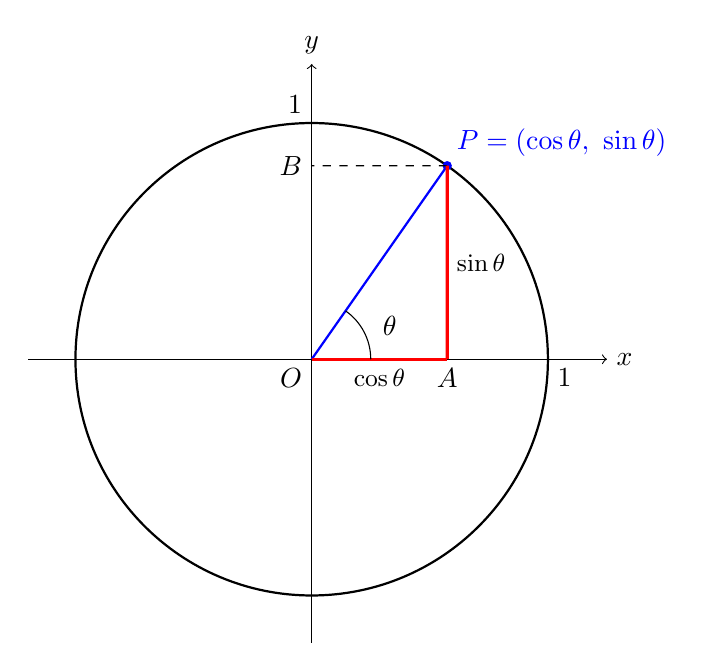
\begin{tikzpicture}[scale=3]
  \draw[->] (-1.2,0) -- (1.25,0) node[right] {$x$};
  \draw[->] (0,-1.2) -- (0,1.25) node[above] {$y$};
  \draw[thick] (0,0) circle(1);
  \coordinate (P) at (55:1);
  \draw[thick, blue] (0,0) -- (P);
  \fill[blue] (P) circle (0.02) node[above right] {$P=(\cos\theta,\ \sin\theta)$};
  \draw[dashed] (P) -- (0,{sin(55)});
  \node[left] at (0,{sin(55)}) {$B$};
  \draw[very thick, red] (0,0) -- ({cos(55)},0);
  \draw[very thick, red] ({cos(55)},0) -- (P);
  \node[below] at ({cos(55)},0) {$A$};
  \node[below] at ({cos(55)/2},0) {\small$\cos\theta$};
  \node[right] at ({cos(55)},{sin(55)/2}) {\small$\sin\theta$};
  \draw (0.25,0) arc[start angle=0,end angle=55,radius=0.25];
  \node at (0.33,0.14) {$\theta$};
  \node[below left] at (0,0) {$O$};
  \node[below right] at (1,0) {$1$};
  \node[above left] at (0,1) {$1$};
\end{tikzpicture}
\end{center}

Энэ ажиглалтаар дурын өнцгийн хувьд тодорхойлолтыг өргөтгөнө.

\begin{definition}[Тригонометр функцүүд]
Дурын $\theta\in\R$ радиан өнцөгт харгалзах нэгж тойргийн цэг $P(x,y)$ бол
\[
\cos\theta:=x,\qquad \sin\theta:=y,\qquad
\tg\theta:=\frac{y}{x}\;(x\neq0),\qquad \ctg\theta:=\frac{x}{y}\;(y\neq0).
\]
Иймд $D(\sin)=D(\cos)=\R$,\;
$D(\tg)=\R\setminus\left\{\tfrac{\pi}{2}+k\pi\mid k\in\mathbb{Z}\right\}$,\;
$D(\ctg)=\R\setminus\{k\pi\mid k\in\mathbb{Z}\}$.
\end{definition}

\begin{remark}
$P$ цэг нэгж тойрог дээр оршдог тул $x^2+y^2=1$, өөрөөр хэлбэл
\[
\boxed{\sin^2\theta+\cos^2\theta=1.}
\]
Үүнээс $-1\le\sin\theta\le1$, $-1\le\cos\theta\le1$ шууд гарна.
\end{remark}

\begin{example}[Үндсэн утгууд]
\[
\renewcommand{\arraystretch}{1.6}
\begin{array}{c|ccccc}
\theta & 0 & \frac{\pi}{6} & \frac{\pi}{4} & \frac{\pi}{3} & \frac{\pi}{2}\\\hline
\sin\theta & 0 & \frac12 & \frac{\sqrt2}{2} & \frac{\sqrt3}{2} & 1\\
\cos\theta & 1 & \frac{\sqrt3}{2} & \frac{\sqrt2}{2} & \frac12 & 0\\
\tg\theta & 0 & \frac{\sqrt3}{3} & 1 & \sqrt3 & \nexists\\
\ctg\theta & \nexists & \sqrt3 & 1 & \frac{\sqrt3}{3} & 0
\end{array}
\]
\end{example}

\begin{example}
$\pi$, $\frac{3\pi}{2}$, $\frac{7\pi}{4}$ радиан өнцөгт харгалзах цэгүүдийн координатыг олж,
$\cos$, $\sin$, $\tg$, $\ctg$ утгуудыг ол.
\begin{center}
\begin{tikzpicture}[scale=2.6]
\draw[->] (-1.2,0) -- (1.2,0) node[below right] {$x$};
\draw[->] (0,-1.2) -- (0,1.2) node[left] {$y$};
\draw[thick] (0,0) circle (1);
\draw[thick, red, ->] (0,0) -- (-1,0);
\node[red, above left] at (-1,0) {$P_\pi=(-1,0)$};
\draw[red, ->] (0.3,0) arc (0:180:0.3);
\draw[thick, blue, ->] (0,0) -- (0,-1);
\node[blue, below right] at (0,-1) {$P_{3\pi/2}=(0,-1)$};
\draw[blue, ->] (0.22,0) arc (0:270:0.22);
\draw[thick, green!50!black, ->] (0,0) -- (315:1);
\node[green!50!black, below right] at (315:1)
     {$P_{7\pi/4}=\left(\tfrac{\sqrt2}{2},-\tfrac{\sqrt2}{2}\right)$};
\draw[green!50!black, ->] (0.14,0) arc (0:315:0.14);
\end{tikzpicture}
\end{center}
Иймд
\[
\renewcommand{\arraystretch}{1.5}
\begin{array}{c|cccc}
 & \cos & \sin & \tg & \ctg \\\hline
\pi & -1 & 0 & 0 & \nexists \\
\frac{3\pi}{2} & 0 & -1 & \nexists & 0 \\
\frac{7\pi}{4} & \frac{\sqrt{2}}{2} & -\frac{\sqrt{2}}{2} & -1 & -1
\end{array}
\]
\end{example}

%--------------------------------------------------------------
\subsection{Үе ба график}
%--------------------------------------------------------------
$\theta$ ба $\theta+2\pi$ өнцгүүдэд нэгж тойргийн нэг ижил цэг харгалзах тул
$\sin(x+2\pi)=\sin x$, $\cos(x+2\pi)=\cos x$. Мөн $\theta+\pi$ өнцөгт $P$-ийн эсрэг
$(-x,-y)$ цэг харгалзах тул $\tg(x+\pi)=\frac{-y}{-x}=\tg x$, $\ctg(x+\pi)=\ctg x$.

\begin{theorem}[Үндсэн үе]
$\sin x$ ба $\cos x$-ийн үндсэн үе $2\pi$, $\tg x$ ба $\ctg x$-ийн үндсэн үе $\pi$.
\end{theorem}
\begin{prof}
$\sin x$-ийн хувьд батлая. $T>0$ үе гэж үзье. $x=0$ үед $\sin T=\sin0=0$ тул $T=k\pi$.
$x=\frac{\pi}{2}$ үед $\sin\!\left(\frac{\pi}{2}+T\right)=1$ тул $T=2m\pi$. Иймд хамгийн бага
эерэг үе нь $2\pi$. $\tg x$-ийн хувьд $\tg T=\tg 0=0$ тул $T=k\pi$ ба $\pi$ нь үе болохыг
дээр харсан. Бусад нь адил.
\end{prof}

\begin{center}
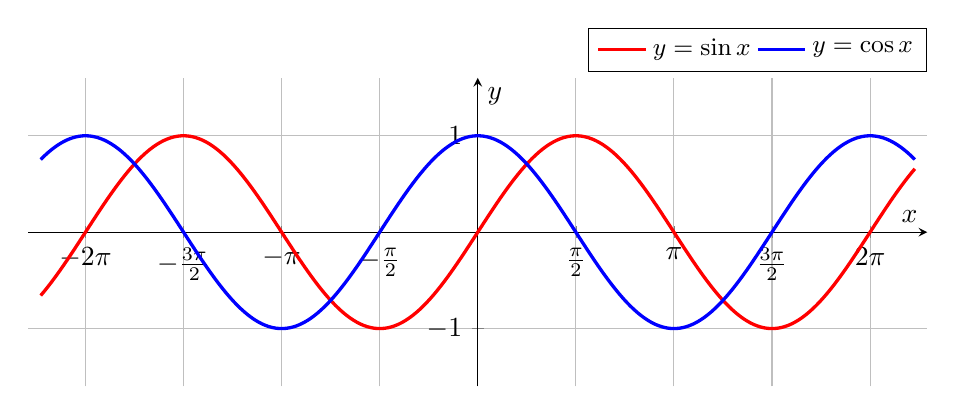
\begin{tikzpicture}
\begin{axis}[
  axis lines=middle, width=13cm, height=5.5cm,
  xmin=-7.2, xmax=7.2, ymin=-1.6, ymax=1.6,
  xlabel={$x$}, ylabel={$y$}, samples=250, domain=-7:7, grid=major,
  xtick={-6.2832,-4.7124,-3.1416,-1.5708,1.5708,3.1416,4.7124,6.2832},
  xticklabels={$-2\pi$,$-\frac{3\pi}{2}$,$-\pi$,$-\frac{\pi}{2}$,$\frac{\pi}{2}$,$\pi$,$\frac{3\pi}{2}$,$2\pi$},
  ytick={-1,1},
  legend style={at={(1,1.02)},anchor=south east,font=\small},legend columns=2]
\addplot[red, very thick] {sin(deg(x))};
\addlegendentry{$y=\sin x$}
\addplot[blue, very thick] {cos(deg(x))};
\addlegendentry{$y=\cos x$}
\end{axis}
\end{tikzpicture}
\end{center}

\begin{center}
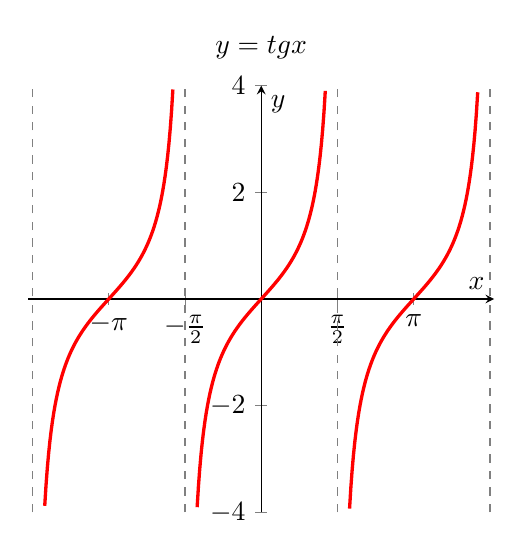
\begin{tikzpicture}
\begin{axis}[
  axis lines=middle, width=7.5cm, height=7cm,
  xmin=-4.8, xmax=4.8, ymin=-4, ymax=4,
  xlabel={$x$}, ylabel={$y$}, samples=100, title={$y=\tg x$},
  xtick={-3.1416,-1.5708,1.5708,3.1416},
  xticklabels={$-\pi$,$-\frac{\pi}{2}$,$\frac{\pi}{2}$,$\pi$}]
\addplot[red, very thick, domain=-4.46:-1.82] {tan(deg(x))};
\addplot[red, very thick, domain=-1.32:1.32] {tan(deg(x))};
\addplot[red, very thick, domain=1.82:4.46] {tan(deg(x))};
\foreach \a in {-4.7124,-1.5708,1.5708,4.7124}
  {\edef\tmp{\noexpand\addplot[gray,dashed] coordinates {(\a,-4) (\a,4)};}\tmp}
\end{axis}
\end{tikzpicture}
\quad
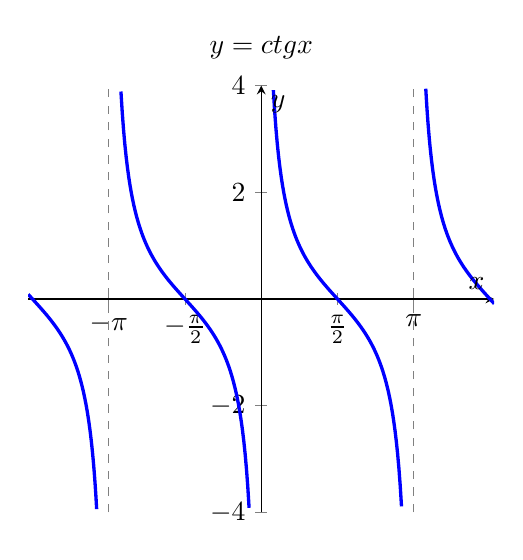
\begin{tikzpicture}
\begin{axis}[
  axis lines=middle, width=7.5cm, height=7cm,
  xmin=-4.8, xmax=4.8, ymin=-4, ymax=4,
  xlabel={$x$}, ylabel={$y$}, samples=100, title={$y=\ctg x$},
  xtick={-3.1416,-1.5708,1.5708,3.1416},
  xticklabels={$-\pi$,$-\frac{\pi}{2}$,$\frac{\pi}{2}$,$\pi$}]
\addplot[blue, very thick, domain=-2.89:-0.25] {cot(deg(x))};
\addplot[blue, very thick, domain=0.25:2.89] {cot(deg(x))};
\addplot[blue, very thick, domain=3.39:4.8] {cot(deg(x))};
\addplot[blue, very thick, domain=-4.8:-3.39] {cot(deg(x))};
\foreach \a in {-3.1416,3.1416}
  {\edef\tmp{\noexpand\addplot[gray,dashed] coordinates {(\a,-4) (\a,4)};}\tmp}
\end{axis}
\end{tikzpicture}
\end{center}

%--------------------------------------------------------------
\subsection{Чухал томьёонууд}
%--------------------------------------------------------------
\textbf{I. Тэгш/сондгой чанар ба үет чанар.}
\begin{align*}
\sin(-x)&=-\sin x, & \cos(-x)&=\cos x, & \tg(-x)&=-\tg x, & \ctg(-x)&=-\ctg x,\\
\sin(x+\pi)&=-\sin x, & \cos(x+\pi)&=-\cos x, &
\sin\!\left(\tfrac{\pi}{2}-x\right)&=\cos x, & \cos\!\left(\tfrac{\pi}{2}-x\right)&=\sin x.
\end{align*}

\textbf{II. Нэмэх томьёо} (баталгааг семинарт хийнэ).
\begin{align*}
\sin(\alpha\pm\beta)&=\sin\alpha\cos\beta\pm\cos\alpha\sin\beta,\\
\cos(\alpha\pm\beta)&=\cos\alpha\cos\beta\mp\sin\alpha\sin\beta.
\end{align*}

\textbf{III. Нийлбэрийг үржвэрт хувиргах томьёо.}
\begin{align*}
\sin x+\sin y&=2\sin\frac{x+y}{2}\cos\frac{x-y}{2}, &
\sin x-\sin y&=2\cos\frac{x+y}{2}\sin\frac{x-y}{2},\\
\cos x+\cos y&=2\cos\frac{x+y}{2}\cos\frac{x-y}{2}, &
\cos x-\cos y&=-2\sin\frac{x+y}{2}\sin\frac{x-y}{2}.
\end{align*}

%--------------------------------------------------------------
\subsection{Тригонометр функцүүдийн чанар}
%--------------------------------------------------------------
\begin{theorem}
$\sin x$ функц $\left[-\frac{\pi}{2};\frac{\pi}{2}\right]$ дээр өсдөг,
$\cos x$ функц $[0;\pi]$ дээр буурдаг,
$\tg x$ функц $\left(-\frac{\pi}{2};\frac{\pi}{2}\right)$ дээр өсдөг,
$\ctg x$ функц $(0;\pi)$ дээр буурдаг.
\end{theorem}
\begin{prof}
$\sin x$-ийн хувьд батлая. $-\frac{\pi}{2}\le a<b\le\frac{\pi}{2}$ бол
\[
\sin b-\sin a=2\cos\frac{a+b}{2}\,\sin\frac{b-a}{2}.
\]
$\frac{b-a}{2}\in\left(0;\frac{\pi}{2}\right]$ тул $\sin\frac{b-a}{2}>0$;
$\frac{a+b}{2}\in\left(-\frac{\pi}{2};\frac{\pi}{2}\right)$ тул $\cos\frac{a+b}{2}>0$.
Иймд $\sin b>\sin a$. Бусад нь үүнтэй адил батлагдана.
\end{prof}

\begin{remark}
$\tg x$ нь интервал бүр дээрээ өсдөг боловч $D(\tg)$ дээр бүхэлдээ өсдөг \itcol{биш}:
$\frac{\pi}{4}<\frac{3\pi}{4}$ боловч $\tg\frac{\pi}{4}=1>-1=\tg\frac{3\pi}{4}$.
\end{remark}

%==============================================================
\section{Тригонометрийн урвуу функцүүд}
%==============================================================
Тригонометр функцүүд үет тул инъектив биш, иймд $\R$ дээр урвуугүй. Лекц 4-т
$x^2$-тай хийсэн шигээ мужийг нь хатуу монотон байх завсраар хязгаарлана.

\begin{definition}
\leavevmode
\begin{itemize}
  \item $\sin:\left[-\frac{\pi}{2};\frac{\pi}{2}\right]\to[-1;1]$ биектив. Урвууг нь
        $\arcsin:[-1;1]\to\left[-\frac{\pi}{2};\frac{\pi}{2}\right]$ гэнэ.
  \item $\cos:[0;\pi]\to[-1;1]$ биектив. Урвууг нь
        $\arccos:[-1;1]\to[0;\pi]$ гэнэ.
  \item $\tg:\left(-\frac{\pi}{2};\frac{\pi}{2}\right)\to\R$ биектив. Урвууг нь
        $\arctg:\R\to\left(-\frac{\pi}{2};\frac{\pi}{2}\right)$ гэнэ.
  \item $\ctg:(0;\pi)\to\R$ биектив. Урвууг нь
        $\arcctg:\R\to(0;\pi)$ гэнэ.
\end{itemize}
Зарим номонд $\sin^{-1}x$, $\tan^{-1}x$ гэж тэмдэглэдэг. Энэ нь $\frac{1}{\sin x}$ \itcol{биш}.
\end{definition}

Өөрөөр хэлбэл
\[
y=\arcsin x \;\Longleftrightarrow\; \sin y=x \text{ ба } y\in\left[-\tfrac{\pi}{2};\tfrac{\pi}{2}\right].
\]

\begin{center}
\begin{tikzpicture}
\begin{axis}[
  axis lines=middle, width=7.5cm, height=7.5cm,
  xmin=-2, xmax=2, ymin=-2, ymax=2,
  xlabel={$x$}, ylabel={$y$}, samples=120, title={$\sin$ ба $\arcsin$},
  legend style={at={(0.02,0.98)},anchor=north west,font=\scriptsize}]
\addplot[red, very thick, domain=-1.5708:1.5708] {sin(deg(x))};
\addlegendentry{$y=\sin x$}
\addplot[blue, very thick, domain=-1:1] {rad(asin(x))};
\addlegendentry{$y=\arcsin x$}
\addplot[gray, dashed, domain=-2:2] {x};
\end{axis}
\end{tikzpicture}
\quad
\begin{tikzpicture}
\begin{axis}[
  axis lines=middle, width=7.5cm, height=7.5cm,
  xmin=-4, xmax=4, ymin=-4, ymax=4,
  xlabel={$x$}, ylabel={$y$}, samples=120, title={$\tg$ ба $\arctg$},
  legend style={at={(0.02,0.98)},anchor=north west,font=\scriptsize}]
\addplot[red, very thick, domain=-1.33:1.33] {tan(deg(x))};
\addlegendentry{$y=\tg x$}
\addplot[blue, very thick, domain=-4:4] {rad(atan(x))};
\addlegendentry{$y=\arctg x$}
\addplot[gray, dashed, domain=-4:4] {x};
\addplot[blue, dotted, domain=-4:4] {1.5708};
\addplot[blue, dotted, domain=-4:4] {-1.5708};
\end{axis}
\end{tikzpicture}
\end{center}

\begin{remark}[Түгээмэл алдаа]
$\sin(\arcsin x)=x$ нь бүх $x\in[-1;1]$-д биелнэ. Харин
$\arcsin(\sin x)=x$ нь зөвхөн $x\in\left[-\frac{\pi}{2};\frac{\pi}{2}\right]$ үед биелнэ:
\[
\arcsin(\sin\pi)=\arcsin 0=0\neq\pi,\qquad
\arcsin\!\left(\sin\tfrac{5\pi}{6}\right)=\arcsin\tfrac12=\tfrac{\pi}{6}.
\]
\end{remark}

\begin{example}[Чанарууд]
\leavevmode
\begin{itemize}
  \item $\arcsin$, $\arctg$ нь сондгой, өсдөг функц:
        $\arcsin(-x)=-\arcsin x$, $\arctg(-x)=-\arctg x$.
  \item $\arccos$, $\arcctg$ нь буурдаг функц бөгөөд
        $\arccos(-x)=\pi-\arccos x$.
  \item $\arctg x$ нь $\R$ дээр тодорхойлогдсон \itcol{зааглагдсан} функц:
        $-\frac{\pi}{2}<\arctg x<\frac{\pi}{2}$.
\end{itemize}
\end{example}

%==============================================================
\section{Илтгэгч ба логарифм функц}
%==============================================================

%--------------------------------------------------------------
\subsection{$e^x$ ба $\ln x$}
%--------------------------------------------------------------
$e\approx2.71828$ тоог хязгаарын бүлэгт нарийвчлан тодорхойлно. $e^x$ функцийн
дараах чанаруудыг одоохондоо баталгаагүй хэрэглэнэ.

\begin{theorem}[Хязгаар ба тасралтгүй чанарын бүлэгт батлагдана]
$f(x)=e^x$ функц
\begin{itemize}
  \item $D=\R$, $E=(0;+\infty)$;
  \item $\R$ дээр өсдөг (иймд инъектив);
  \item $(0;+\infty)$-ийн дурын $y$ тооны хувьд $e^x=y$ байх $x$ олдоно (сюръектив);
  \item $e^{x+y}=e^xe^y$, \; $e^0=1$.
\end{itemize}
\end{theorem}

Иймд $e^x:\R\to(0;+\infty)$ биектив тул урвуутай.

\begin{definition}[Натурал логарифм]
$e^x:\R\to(0;+\infty)$ функцийн урвууг \itcol{натурал логарифм} гээд
$\ln:(0;+\infty)\to\R$ гэж тэмдэглэнэ:
\[
y=\ln x \;\Longleftrightarrow\; e^y=x.
\]
Иймд $\ln(e^x)=x$ \;($x\in\R$), \; $e^{\ln x}=x$ \;($x>0$).
\end{definition}

\begin{center}
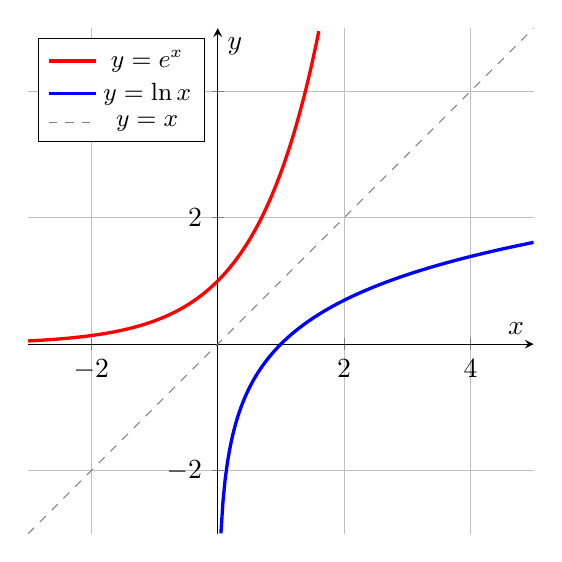
\begin{tikzpicture}
\begin{axis}[
  axis lines=middle, width=8cm, height=8cm,
  xmin=-3, xmax=5, ymin=-3, ymax=5,
  xlabel={$x$}, ylabel={$y$}, samples=150, grid=major,
  legend style={at={(0.02,0.98)},anchor=north west,font=\small}]
\addplot[red, very thick, domain=-3:1.6] {exp(x)};
\addlegendentry{$y=e^x$}
\addplot[blue, very thick, domain=0.05:5] {ln(x)};
\addlegendentry{$y=\ln x$}
\addplot[gray, dashed, domain=-3:5] {x};
\addlegendentry{$y=x$}
\end{axis}
\end{tikzpicture}
\end{center}

\begin{theorem}
$x,y>0$, $r\in\R$ бол
\[
\ln(xy)=\ln x+\ln y,\qquad \ln\frac{x}{y}=\ln x-\ln y,\qquad \ln 1=0.
\]
\end{theorem}
\begin{prof}
$u=\ln x$, $v=\ln y$ гэвэл $e^u=x$, $e^v=y$ тул $e^{u+v}=e^ue^v=xy$. Логарифмын
тодорхойлолтоор $\ln(xy)=u+v$. Бусад нь адил.
\end{prof}

\begin{remark}[Түгээмэл алдаа]
$\ln(x^2)=2\ln x$ нь зөвхөн $x>0$ үед зөв. $x\neq0$ бүрд $\ln(x^2)=2\ln|x|$.
\end{remark}

%--------------------------------------------------------------
\subsection{$a^x$, $\log_a x$ ба зэрэгт функц}
%--------------------------------------------------------------
\begin{definition}
$a>0$, $a\neq1$ байг.
\[
a^x:=e^{x\ln a}\quad(x\in\R),\qquad
\log_a x:=\frac{\ln x}{\ln a}\quad(x>0),\qquad
x^\alpha:=e^{\alpha\ln x}\quad(x>0,\ \alpha\in\R).
\]
\end{definition}

\begin{remark}
Эндээс $a^x$-ийг $e$ суурьтай илтгэгч рүү шилжүүлж болно. Жишээ нь
$3^x=e^{x\ln3}\approx e^{1.0986\,x}$. Тиймээс анализад голчлон $e^x$, $\ln x$-ийг ашигладаг.
Мөн $\log_a x$ нь $a^x$-ийн урвуу функц: $\log_a(a^x)=x$, \; $a^{\log_a x}=x$.
\end{remark}

\textbf{Илтгэгч функцийн чанарууд} ($a,b>0$, $x,y\in\R$):
\[
a^0=1,\quad a^xa^y=a^{x+y},\quad \frac{a^x}{a^y}=a^{x-y},\quad (a^x)^y=a^{xy},\quad
(ab)^x=a^xb^x,\quad \left(\frac ab\right)^x=\frac{a^x}{b^x}.
\]

\textbf{Логарифм функцийн чанарууд} ($a,b>0$, $a,b\neq1$, $x,y>0$, $r\in\R$):
\[
\log_a1=0,\quad \log_aa=1,\quad \log_a(xy)=\log_ax+\log_ay,\quad
\log_a\frac xy=\log_ax-\log_ay,
\]
\[
\log_a(x^r)=r\log_ax,\qquad \log_ax=\frac{\log_bx}{\log_ba}\ \text{(суурь солих томьёо)}.
\]

\begin{theorem}[Монотон чанар]
$a>1$ бол $a^x$ нь $\R$ дээр, $\log_ax$ нь $(0;+\infty)$ дээр өсдөг.
$0<a<1$ бол хоёулаа буурдаг.
\end{theorem}
\begin{prof}
$a>1$ бол $\ln a>0$ тул $x\mapsto x\ln a$ өсдөг. Өсдөг хоёр функцийн нийлмэл
$e^{x\ln a}$ мөн өсдөг. $0<a<1$ бол $\ln a<0$ тул $x\ln a$ буурдаг, иймд $a^x$ буурдаг.
$\log_ax=\frac{\ln x}{\ln a}$-ийн хувьд ч адил.
\end{prof}

\begin{remark}
$a>1$ үед $a^x\to0$ ($x\to-\infty$), $a^x\to+\infty$ ($x\to+\infty$);
$\log_ax\to-\infty$ ($x\to0^+$), $\log_ax\to+\infty$ ($x\to+\infty$).
Эдгээрийг хязгаарын бүлэгт баталгаатай үзнэ.
\end{remark}

%==============================================================
\section{Үндсэн элементар функцүүдийн нэгтгэл}
%==============================================================
\begin{definition}
Тогтмол, зэрэгт, илтгэгч, логарифм, тригонометр ба урвуу тригонометр функцүүдийг
\itcol{үндсэн элементар функц} гэнэ. Эдгээрээс арифметик үйлдэл болон нийлмэл функц
авах үйлдлийг төгсгөлөг удаа хэрэглэж гаргасан функцийг \itcol{элементар функц} гэнэ.
\end{definition}

\begin{center}
\small
\renewcommand{\arraystretch}{1.4}
\begin{tabular}{c|c|c|c|c|c}
Функц & $D(f)$ & $E(f)$ & Тэгш/сондгой & Монотон & Зааглагдсан\\\hline
$x^2$ & $\R$ & $[0;+\infty)$ & тэгш & биш & доороос\\
$x^3$ & $\R$ & $\R$ & сондгой & өсдөг & үгүй\\
$\frac1x$ & $\R\setminus\{0\}$ & $\R\setminus\{0\}$ & сондгой & биш$^{*}$ & үгүй\\\hline
$\sin x$ & $\R$ & $[-1;1]$ & сондгой & биш & тийм\\
$\cos x$ & $\R$ & $[-1;1]$ & тэгш & биш & тийм\\
$\tg x$ & $x\neq\frac{\pi}{2}+k\pi$ & $\R$ & сондгой & биш$^{*}$ & үгүй\\\hline
$\arcsin x$ & $[-1;1]$ & $\left[-\frac{\pi}{2};\frac{\pi}{2}\right]$ & сондгой & өсдөг & тийм\\
$\arccos x$ & $[-1;1]$ & $[0;\pi]$ & аль ч биш & буурдаг & тийм\\
$\arctg x$ & $\R$ & $\left(-\frac{\pi}{2};\frac{\pi}{2}\right)$ & сондгой & өсдөг & тийм\\\hline
$e^x$ & $\R$ & $(0;+\infty)$ & аль ч биш & өсдөг & доороос\\
$\ln x$ & $(0;+\infty)$ & $\R$ & хамаарахгүй & өсдөг & үгүй
\end{tabular}

\smallskip
{\footnotesize $^{*}$ Тодорхойлогдох мужийн интервал бүр дээр хатуу монотон.}
\end{center}

%==============================================================
\section{Дараалал}
%==============================================================
\begin{definition}
$f:\N\to\R$ функцийг \itcol{тоон дараалал} гэнэ.
\end{definition}
Дараалал нь $f(1)=a_1$, $f(2)=a_2$, $f(3)=a_3,\ldots$ утгуудаар бүрэн тодорхойлогдох тул
$f$-г $a_1,a_2,a_3,\ldots$ эсвэл $\{a_n\}$ гэж тэмдэглэнэ.

\begin{example}
$f(n)=2n+1$ дарааллыг $a_n=2n+1$ гэж бичнэ: $3,5,7,9,\ldots$
\end{example}

\itcol{Санамж.} Дараалал нь функц учир монотон, өсдөг, буурдаг, зааглагдсан гэх мэт
нэр томьёог шууд хэрэглэнэ.

\begin{example}
$a_n=n$ дараалал өсдөг, доороосоо зааглагдсан ($a_n\ge1$), дээрээсээ зааглагдаагүй.
\end{example}

Дарааллыг дараах хоёр аргаар өгдөг.
\begin{description}
  \item[a)] \itcol{Ерөнхий гишүүний томьёо} — дурын гишүүнийг $n$-ээр шууд илэрхийлнэ.
            Жишээ нь $a_n=3n-2$.
  \item[b)] \itcol{Рекуррент томьёо} — гишүүнийг өмнөх гишүүдээр нь илэрхийлнэ.
            Жишээ нь $a_1=1$, $a_{n+1}=a_n+3$.
\end{description}

%--------------------------------------------------------------
\subsection{Арифметик прогресс}
%--------------------------------------------------------------
\begin{definition}[Арифметик прогресс]
$\forall n\in\N$ хувьд $a_{n+1}=a_n+d$ байвал $\{a_n\}$-г \itcol{арифметик прогресс},
$d$-г түүний \itcol{ялгавар} гэнэ.
\end{definition}

Ерөнхий гишүүн: $a_n=a_1+(n-1)d$.

\begin{example}
$a_1=3$, $d=4$ бол $3,7,11,15,19,\ldots$ ба $a_n=3+(n-1)\cdot4=4n-1$.
\end{example}

\begin{example}
$a_3=11$, $a_7=27$ бол $a_1+2d=11$, $a_1+6d=27$. Хасвал $4d=16$, иймд $d=4$, $a_1=3$,
$a_n=4n-1$.
\end{example}

\begin{theorem}[Эхний $k$ гишүүний нийлбэр]
$S_k=a_1+a_2+\dots+a_k$ бол
\[
S_k=\frac{k(a_1+a_k)}{2}=\frac{k\bigl(2a_1+(k-1)d\bigr)}{2}.
\]
\end{theorem}
\begin{prof}
Математик индукцээр батлая.

\textbf{Суурь} ($k=1$): $S_1=a_1=\dfrac{1\cdot(2a_1+0)}{2}$.

\textbf{Алхам.} $k=m$ үед томьёо биелнэ гэж үзвэл
\begin{align*}
S_{m+1}&=S_m+a_{m+1}=\frac{m\bigl(2a_1+(m-1)d\bigr)}{2}+a_1+md\\
&=\frac{2a_1(m+1)+d\bigl(m(m-1)+2m\bigr)}{2}=\frac{(m+1)(2a_1+md)}{2}.
\end{align*}
Энэ нь $k=m+1$ үеийн томьёо тул бүх $k\in\N$-д биелнэ.
\end{prof}

%--------------------------------------------------------------
\subsection{Геометр прогресс}
%--------------------------------------------------------------
\begin{definition}[Геометр прогресс]
$a_n\neq0$ ба $\forall n\in\N$ хувьд $a_{n+1}=a_nq$ байвал $\{a_n\}$-г
\itcol{геометр прогресс}, $q$-г түүний \itcol{хуваарь} гэнэ.
\end{definition}

Ерөнхий гишүүн: $a_n=a_1q^{n-1}$.

\begin{example}
$a_1=2$, $q=3$ бол $2,6,18,54,162,\ldots$ ба $a_n=2\cdot3^{n-1}$.
\end{example}

\begin{example}
$a_2=6$, $a_5=162$ бол $a_1q=6$, $a_1q^4=162$. Хуваавал $q^3=27$, иймд $q=3$, $a_1=2$.
\end{example}

\begin{theorem}[Эхний $k$ гишүүний нийлбэр]
\[
S_k=
\begin{cases}
\dfrac{a_1(q^k-1)}{q-1}, & q\neq1,\\[6pt]
k\,a_1, & q=1.
\end{cases}
\]
\end{theorem}
\begin{prof}
$q=1$ бол бүх гишүүн $a_1$ тул $S_k=ka_1$. $q\neq1$ үед индукцээр батлая.
$S_1=a_1=\dfrac{a_1(q-1)}{q-1}$. $k=m$ үед биелнэ гэж үзвэл
\[
S_{m+1}=\frac{a_1(q^m-1)}{q-1}+a_1q^m=\frac{a_1\bigl(q^m-1+q^{m+1}-q^m\bigr)}{q-1}
=\frac{a_1(q^{m+1}-1)}{q-1}.
\]
\end{prof}

%--------------------------------------------------------------
\subsection{Арифметик-геометр прогресс}
%--------------------------------------------------------------
\begin{definition}
$q,d\in\R$ байхад $a_{n+1}=q\,a_n+d$ рекуррент томьёогоор тодорхойлогдох $\{a_n\}$-г
\itcol{арифметик-геометр прогресс} гэнэ.
\end{definition}

\begin{remark}
$q=1$ бол $d$ ялгавартай арифметик прогресс, $d=0$ бол $q$ хуваартай геометр прогресс.
\end{remark}

$q\neq1$ үед ерөнхий гишүүнийг олъё. $a_{n+1}-c=q(a_n-c)$ байх $c$ тоог хайвал
$a_{n+1}=qa_n+c(1-q)$ тул $c(1-q)=d$, өөрөөр хэлбэл $c=\dfrac{d}{1-q}$.
$b_n=a_n-c$ гэвэл $b_{n+1}=qb_n$ тул $\{b_n\}$ геометр прогресс ба $b_n=b_1q^{n-1}$. Иймд
\[
\boxed{a_n=\frac{d}{1-q}+\left(a_1-\frac{d}{1-q}\right)q^{n-1}.}
\]

\begin{example}
$a_1=2$, $a_{n+1}=2a_n-3$.
\begin{enumerate}
  \item Гишүүдийг цувуулан бичвэл $a_2=1$, $a_3=-1$, $a_4=-5$, $a_5=-13$, $a_6=-29$, $a_7=-61$.
  \item $a_{n+1}-c=2(a_n-c)$-ийг задалбал $a_{n+1}=2a_n-c$ тул $c=3$.
  \item $b_n=a_n-3$ гэвэл $b_1=-1$, $b_{n+1}=2b_n$ тул $b_n=-2^{n-1}$.
  \item Иймд $\boxed{a_n=3-2^{n-1}}$. \; Шалгалт: $a_7=3-64=-61$. \checkmark
\end{enumerate}
\end{example}

\begin{example}
$a_1=5$, $a_{n+1}=3a_n+4$. Энд $q=3$, $d=4$ тул $c=\dfrac{4}{1-3}=-2$.
$b_n=a_n+2$ гэвэл $b_1=7$, $b_n=7\cdot3^{n-1}$. Иймд $\boxed{a_n=7\cdot3^{n-1}-2.}$
\end{example}

%##############################################################
\section{Семинар ба гэрийн даалгавар (Лекц 5)}
%##############################################################

%--------------------------------------------------------------
\subsection*{A. Тригонометрийн адилтгалууд}
%--------------------------------------------------------------
$O(0,0)$ төвтэй нэгж тойрог дээрх $\alpha$ радиан өнцөгт харгалзах $P(\alpha)$ цэг
$(\cos\alpha;\ \sin\alpha)$ координаттай ба $\cos^2\alpha+\sin^2\alpha=1$.

\begin{center}
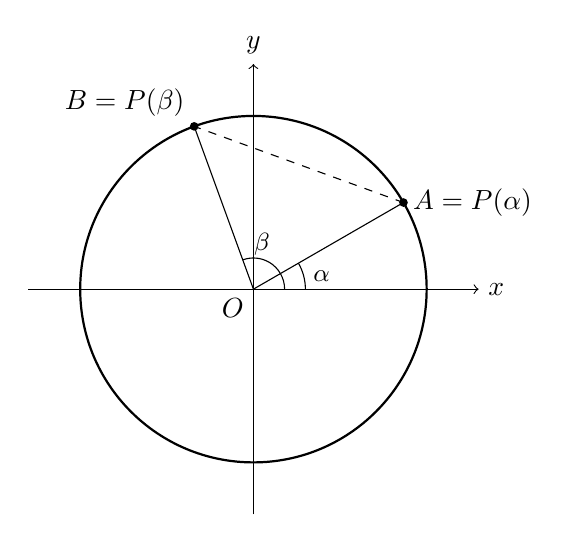
\begin{tikzpicture}[scale=2.2]
  \draw[->] (-1.3,0) -- (1.3,0) node[right] {$x$};
  \draw[->] (0,-1.3) -- (0,1.3) node[above] {$y$};
  \draw[thick] (0,0) circle (1);
  \coordinate (O) at (0,0);
  \coordinate (A) at (30:1);
  \coordinate (B) at (110:1);
  \draw (O) -- (A) (O) -- (B);
  \draw[dashed] (A) -- (B);
  \fill (A) circle (0.025) node[right] {$A=P(\alpha)$};
  \fill (B) circle (0.025) node[above left] {$B=P(\beta)$};
  \node[below left] at (O) {$O$};
  \draw (0.3,0) arc (0:30:0.3) node[midway,right] {\small$\alpha$};
  \draw (0.18,0) arc (0:110:0.18);
  \node at (0.05,0.26) {\small$\beta$};
\end{tikzpicture}
\end{center}

\begin{enumerate}
\item
\begin{enumerate}[label=\alph*)]
  \item $P(0)$, $P\!\left(\frac{\pi}{4}\right)$, $P\!\left(\frac{\pi}{3}\right)$,
        $P\!\left(\frac{\pi}{2}\right)$, $P(\pi)$ цэгүүдийг ашиглан харгалзах өнцгийн
        косинус, синусыг тооцоол.
  \item $P(\alpha)=A$, $P(\beta)=B$ байг. $\sqrt{(x_1-x_2)^2+(y_1-y_2)^2}$ томьёогоор $|AB|$-г ол.
  \item $AOB$ гурвалжинд косинусын теорем хэрэглэн $|AB|$-г ол.
  \item $\cos(\alpha-\beta)=\cos\alpha\cos\beta+\sin\alpha\sin\beta$ гэж батал.
  \item $\cos\!\left(\frac{\pi}{2}-x\right)=\sin x$, \; $\sin\!\left(\frac{\pi}{2}-x\right)=\cos x$ гэж батал.
  \item $\sin(\alpha+\beta)=\sin\alpha\cos\beta+\cos\alpha\sin\beta$ гэж батал.
\end{enumerate}
\item
\begin{enumerate}[label=\alph*)]
  \item $\sin2x=2\sin x\cos x$ гэж батал.
  \item $\cos2x=1-2\sin^2x$ гэж батал.
  \item $\alpha=60^\circ$, $\beta=30^\circ$ үед $\cos(\alpha-\beta)$-ийн томьёог шалга.
  \item $\tg2x$-ийг $\tg x$-ээр илэрхийл.
\end{enumerate}
\item $s(x)=\sin x-\cos x$ функцийг $a\sin(x+\varphi)$ хэлбэрт бичиж, утгын мужийг ол.
\end{enumerate}

%--------------------------------------------------------------
\subsection*{B. Урвуу тригонометр, илтгэгч ба логарифм}
%--------------------------------------------------------------
\begin{enumerate}[resume]
\item $\arcsin\frac12$, \; $\arccos\frac12$, \; $\arctg1$, \; $\arcsin\!\left(\sin\frac{7\pi}{6}\right)$-ийн утгыг ол.
\item $x\in[-1;1]$ бол $\arcsin x+\arccos x=\dfrac{\pi}{2}$ гэж батал.
\item $h(x)=\arccos x$ функцийн утгын мужийг бич.
\item
\begin{enumerate}[label=\alph*)]
  \item $\ln(e^x)=x$ ба $e^{\ln x}=x$ ($x>0$) гэж батал.
  \item $x>0$ бол $\ln\sqrt{x}=\frac12\ln x$ гэж батал.
\end{enumerate}
\item $g(x)=\log_2(x-3)$ функцийн тодорхойлогдох мужийг ол.
\end{enumerate}

%--------------------------------------------------------------
\subsection*{C. Тодорхойлогдох муж}
%--------------------------------------------------------------
\begin{enumerate}[resume]
\item Дараах функцийн тодорхойлогдох мужийг ол.
\begin{enumerate}
  \item $y=\log_{x+1}(x^2-3x+2)$
  \item $y=\log_6\log_{0.5}(4-x)$
  \item $y=\sqrt{5x^2-3x+23}+\lg(x^2-10x+16)+\dfrac1x$
  \item $y=\sqrt{\log_{0.5}\log_3\dfrac{x+1}{x-1}}$
  \item $y=\sqrt{x^2-3x-10}\,\lg|x-3|$
  \item $y=\sqrt{\log_{5-x}(x^2-9)}$
  \item $y=\arccos\!\left(\dfrac{|x-1|}{x-1}+\dfrac{|x-2|}{x-2}+\dfrac{|x-3|}{x-3}\right)$
  \item $y=\arcsin\dfrac{\frac x3-\frac3x}{2}$
  \item $y=\lg(\arcsin(\lg x))$
  \item $f(x)=\sqrt{\arcsin x-\arccos x}$
  \item $f(x)=\sqrt{\arccos\dfrac{3x+1}{5}-\arcsin\dfrac{x+2}{5}}$
  \item $f(x)=\sqrt{\dfrac{5\pi}{6}-\arcsin(2x)-\arccos(6x-2)}$
  \item $f(x)=\sqrt{\dfrac{3\pi}{4}-\arccos x-\arccos(x\sqrt2)-\arccos(x\sqrt3)}$
  \item $f(x)=\sqrt{\sin(\cos x)}$
  \item $f(x)=\sqrt{\sin\sqrt{x}}$
  \item $f(x)=\sqrt{\tg^2x-(\sqrt3+1)\tg x+\sqrt3}$
\end{enumerate}
\end{enumerate}

%--------------------------------------------------------------
\subsection*{D. Утгын муж}
%--------------------------------------------------------------
\begin{enumerate}[resume]
\item Дараах функцүүдийн утгын мужийг ол.
\begin{enumerate}
  \item $f(x)=\sqrt{\dfrac{\sin3x\cos\left(2x-\frac{\pi}{6}\right)}{\sin2x}}$
  \item $f(x)=\sqrt{\cos3x+\sin x\sin2x}$
  \item $f(x)=\sqrt{\sin5x-\cos3x}$
  \item $f(x)=\sqrt{\dfrac{\cos3x}{\sin3x-2\sin x}}-\tg x$
  \item $f(x)=\cos^2x+\cos x+3$
  \item $f(x)=\sin^2x-4\sin x+3$
  \item $f(x)=2^{x^2+4x+5}$
  \item $f(x)=\log_3(5+4x-x^2)$
  \item $f(x)=\sqrt{2\lg x-(\lg x)^2}$
  \item $f(x)=\sin x-5\cos x$
  \item $f(x)=\dfrac{\sin x-\cos x}{\sin x+\cos x}$
  \item $f(x)=\log_2(\cos x+\sin^2x)$
\end{enumerate}
\end{enumerate}

%--------------------------------------------------------------
\subsection*{E. Урвуу функц}
%--------------------------------------------------------------
\begin{enumerate}[resume]
\item Урвуу функцийг ол.
\begin{enumerate}
  \item $y=2^{x^2-2x}$, \; $x\in(-\infty;1]$
  \item $y=1-e^{\frac{1-x}{1+x}}$, \; $x\in\R\setminus\{-1\}$
  \item $y=\dfrac{3^x-2^x}{3^x+2^x}$, \; $x\in\R$
  \item $y=\log_2\!\left(x+\sqrt{x^2+1}\right)$, \; $x\in\R$
  \item $y=\sin x$, \; $x\in\left[-\frac{3\pi}{2};-\frac{\pi}{2}\right]$
  \item $y=\sin x$, \; $x\in\left[\frac{\pi}{2};\frac{3\pi}{2}\right]$
  \item $y=\cos x$, \; $x\in[-\pi;0]$
  \item $y=\cos x$, \; $x\in[2\pi;3\pi]$
\end{enumerate}
\end{enumerate}

%--------------------------------------------------------------
\subsection*{F. График}
%--------------------------------------------------------------
\begin{enumerate}[resume]
\item Дараах функцүүдийн графикийг дүрсэл.
\begin{enumerate}
  \item $f(x)=\sin^4x-\cos^4x$
\end{enumerate}
\end{enumerate}

%--------------------------------------------------------------
\subsection*{G. Дараалал}
%--------------------------------------------------------------
\begin{enumerate}[resume]
\item $a_n=n^2+1$ дарааллын эхний 5 гишүүнийг ол.
\item $a_1=2$, $a_{n+1}=a_n+5$ бол $a_5$ ба ерөнхий гишүүн $a_n$-ийг ол.
\item $a_n=\dfrac{3n+1}{2n+5}$ бол $a_1,a_2,a_3$-ийг олж, $\{a_n\}$ өсдөг эсэхийг шалга.
      Зааглагдсан эсэхийг тогтоо.
\item $a_n=\dfrac1n$ дараалал буурдгийг батал. Доороосоо болон дээрээсээ зааглагдсан эсэхийг тогтоо.
\end{enumerate}